%%%%%%%%%%%%%%%%%%%%%%%%%%%%%%%%%%%%%%%%%
% Journal Article
% LaTeX Template
% Version 1.4 (15/5/16)
%
% This template has been downloaded from:
% http://www.LaTeXTemplates.com
%
% Original author:
% Frits Wenneker (http://www.howtotex.com) with extensive modifications by
% Vel (vel@LaTeXTemplates.com)
%
% License:
% CC BY-NC-SA 3.0 (http://creativecommons.org/licenses/by-nc-sa/3.0/)
%
%%%%%%%%%%%%%%%%%%%%%%%%%%%%%%%%%%%%%%%%%

%----------------------------------------------------------------------------------------
%	PACKAGES AND OTHER DOCUMENT CONFIGURATIONS
%----------------------------------------------------------------------------------------

\documentclass[twoside,twocolumn]{article}

\usepackage{blindtext} % Package to generate dummy text throughout this template 
%\usepackage[utf8]{inputenc} % Package for unicode characters
\usepackage[utf8]{inputenc}
\usepackage{amssymb}
\usepackage{newunicodechar}
\newunicodechar{Ɖ}{\DH}

\usepackage[sc]{mathpazo} % Use the Palatino font
\usepackage[T1]{fontenc} % Use 8-bit encoding that has 256 glyphs
\linespread{1.05} % Line spacing - Palatino needs more space between lines
\usepackage{microtype} % Slightly tweak font spacing for aesthetics

\usepackage[english]{babel} % Language hyphenation and typographical rules

\usepackage[hmarginratio=1:1,top=32mm,columnsep=20pt]{geometry} % Document margins
\usepackage[hang, small,labelfont=bf,up,textfont=it,up]{caption} % Custom captions under/above floats in tables or figures
\usepackage{booktabs} % Horizontal rules in tables

\usepackage{lettrine} % The lettrine is the first enlarged letter at the beginning of the text
\usepackage{url} %added by John Domingue
\usepackage{graphicx} % added by John Domingue
\graphicspath{ {tex/images/} }
\usepackage{enumitem} % Customized lists
\setlist[itemize]{noitemsep} % Make itemize lists more compact

\usepackage{abstract} % Allows abstract customization
\renewcommand{\abstractnamefont}{\normalfont\bfseries} % Set the "Abstract" text to bold
\renewcommand{\abstracttextfont}{\normalfont\small\itshape} % Set the abstract itself to small italic text

\usepackage{titlesec} % Allows customization of titles
\renewcommand\thesection{\Roman{section}} % Roman numerals for the sections
\renewcommand\thesubsection{\roman{subsection}} % roman numerals for subsections
\titleformat{\section}[block]{\large\scshape\centering}{\thesection.}{1em}{} % Change the look of the section titles
\titleformat{\subsection}[block]{\large}{\thesubsection.}{1em}{} % Change the look of the section titles

\usepackage{fancyhdr} % Headers and footers
\pagestyle{fancy} % All pages have headers and footers
\fancyhead{} % Blank out the default header
\fancyfoot{} % Blank out the default footer
\fancyhead[C]{Ethereum Classic Library $\bullet$ October 2016 $\bullet$ Vol. I, No. 1} % Custom header text
\fancyfoot[RO,LE]{\thepage} % Custom footer text

\usepackage{titling} % Customizing the title section

\usepackage[pagebackref]{hyperref} % For hyperlinks in the PDF

%----------------------------------------------------------------------------------------
%	TITLE SECTION
%----------------------------------------------------------------------------------------
\setlength{\droptitle}{-4\baselineskip} % Move the title up

\pretitle{\begin{center}\Huge\bfseries} % Article title formatting
\posttitle{\end{center}} % Article title closing formatting
\title{Blockchain Library Whitepaper} % Article title
\author{%
\textsc{Prophet Daniel}\thanks{The author would like to thank the Ethereum Classic community.} \\[1ex] % Your name
\normalsize University of Nicosia \\ % Your institution
\normalsize \href{mailto:prophetdaniel@ethereumclassic.org}{prophetdaniel@ethereumclassic.org} % Your email address
\and % Uncomment if 2 authors are required, duplicate these 4 lines if more
\textsc{John Domingue}\thanks{} \\[1ex] % Second author's
\normalsize Knowledge Media Institute, Open University \\ % Second author's institution
\normalsize \href{mailto:John.domingue@open.ac.uk}{John.domingue@open.ac.uk} % Second
% author's email address
}
\date{\today} % Leave empty to omit a date
\renewcommand{\maketitlehookd}{%
\begin{abstract}
\noindent In this paper a blockchain library organization is proposed for
increasing the community awareness of the blockchain technology and fulfilling
the gaps needed to deliver benefits to society from its application.  
\end{abstract}
}

%----------------------------------------------------------------------------------------

\begin{document}

% Print the title
\maketitle

%----------------------------------------------------------------------------------------
%	ARTICLE CONTENTS
%----------------------------------------------------------------------------------------

\section{Introduction}

\begin{itemize}
	\item What blockchains are and why they are important
	\item Although there is a lot of available information on technical aspects
	of blockchains there is no coherent space for on blockchain applications
	\item Although there is a lot of available information on technical aspects
	of blockchains there is no coherent space for on blockchain applications
	\item Need to bring the developer, research and policy
	communities together (may also others)
	\item Proposal of this paper
\end{itemize}

% \lettrine[nindent=0em,lines=3]{A} decentralized autonomous organization (DAO) is an organization that is run through rules encoded as computer programs called smart contracts and its financial transaction record and program rules are maintained on a blockchain.
% The most famous DAO up to date has as purpose venture capital funding and is called The DAO, which was launched with US\$150 million in crowdfunding in May 2016 and was hacked and drained of approximately US\$50 million in cryptocurrency three weeks later \cite{Price2016}.\par 
% On May 26th of 2016, a paper\cite{Popper2016} first pointed out system vulnerabilities in the operation of The DAO, and recommended a temporary moratorium until all security breaches were fixed. Since its publication and the hack on June 17th, other system vulnerabilities were also found. The hacker had 22 days to study these points, collect all possibilities and take action.\par
% Security breaches are often found by specialists\cite{Perlroth2014}, then publicized as an alerting mechanism to avoid making harm to people. After that happens, hackers are motivated by the amount of money at stake to take action, and they often do way before the fix is deployed.\par
% The DAO was not engineered smart enough to deal with this specific problem. Actually it was not smart in the sense of smartness as we know it. Contrary to what the name suggests, it is also not autonomous yet, because whenever a smart decision needs to be taken, The DAO relies on a voting mechanism to reach its ultimate goal, where the more tokens the voter holds, the more voting power is given to it. In other words, The DAO utilizes human collective intelligence to decide therefore it should be called DO rather than DAO.
\cite{kurzweil2000age}

%------------------------------------------------
\section{The Blockchain Library organization}

\subsection{Blockchain Library vision}

\subsection{Library Shelf}
Aggregation of blockchain application documents

\subsection{Development Platform}
Space that allows the development of new whitepapers of blockchain applications.
 
\subsection{State of the art} 
The earliest library consisting of collections of clay tablets in cuneiform
script date back to 2600 BC %\cite{History_of_Libraries2016}. Through the
% Library of Alexandria (3BC) up until the 1960s libraries existed as collections of
physical information sources. Conceptually, one of the main contributions in the
history of the preservation of human knowledge came from Vannevar Bush and his
famous 1945 essay ``As We May Think". This paper predicted many technologies in
widespread use today including hypertext,PC, the Internet and Web and online
encyclopedias %\cite{As_We_May_Think2016}. Vannevar envisioned the Memex: a
collective knowledge store where words and phrases are linked to associated
other terms. Doug Engelbart pursued this vision when in 1968 he gave the
``Mother of All Demos" %\cite{Mother_of_All_Demos2016} demonstrating for the
first time windows, hypertext, word processing, dynamic file linking and
collaborative work.

For the most part digital libraries today and scholarly papers tend to replicate
the established structure of a library consisting of publications. Publications
may contain references to other publications. ScholOnto
%\cite{shum2000scholonto, Scholonto2016} was one of the first projects to imagine and construct native Web
scholarly publishing. The main outcome of this project the notion of a scholarly
claim which linked an author to an assertion (a relationship between two
concepts or documents or between a concept or document and another claim)
supported by a justification.

\begin{figure}[htbp]\centering
\caption{All claims are owned by an agent and have some form of justification.
Claims assert relationships with other claims or between concepts. (taken from shum2000scholonto).}
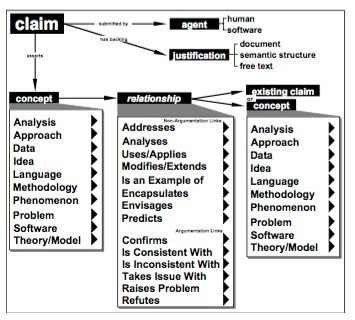
\includegraphics[width=0.46\textwidth]{scholonto-image}
\label{fig:scholonto}

\end{figure}

todo 
Micropublications
RASH
Open Access Libraries

 
\subsection{Innovation Drive} 
Embed blockchain publications into a wider startup and innovation ecosystem
(e.g. allow for concepts/work to be attributable)
 
\section{Conclusion}
\Blindtext

%Maecenas sed ultricies felis. Sed imperdiet dictum arcu a egestas. 
%\begin{itemize}
%\item Donec dolor arcu, rutrum id molestie in, viverra sed diam
%\item Curabitur feugiat
%\item turpis sed auctor facilisis
%\item arcu eros accumsan lorem, at posuere mi diam sit amet tortor
%\item Fusce fermentum, mi sit amet euismod rutrum
%\item sem lorem molestie diam, iaculis aliquet sapien tortor non nisi
%\item Pellentesque bibendum pretium aliquet
%\end{itemize}
%\blindtext % Dummy text

%Text requiring further explanation\footnote{Example footnote}.

%------------------------------------------------

%\section{Results}

%\begin{table}
%\caption{Example table}
%\centering
%\begin{tabular}{llr}
%\toprule
%\multicolumn{2}{c}{Name} \\
%\cmidrule(r){1-2}
%First name & Last Name & Grade \\
%\midrule
%John & Doe & $7.5$ \\
%Richard & Miles & $2$ \\
%\bottomrule
%\end{tabular}
%\end{table}

%\blindtext % Dummy text

%\begin{equation}
%\label{eq:emc}
%e = mc^2
%\end{equation}

%\blindtext % Dummy text

%------------------------------------------------

%\section{Discussion}

%\subsection{Subsection One}

%A statement requiring citation \cite{Figueredo2009}.
%\blindtext % Dummy text

%\subsection{Subsection Two}

%\blindtext % Dummy text

%----------------------------------------------------------------------------------------
%	REFERENCE LIST
%----------------------------------------------------------------------------------------

\bibliographystyle{abbrv}  
\bibliography{bibliography}

%----------------------------------------------------------------------------------------

\end{document}
